% main.tex
% header.tex
\documentclass[a4paper,11pt,twoside,ngerman,color]{article}
\usepackage[a4paper,left=3.5cm,right=2.5cm,bottom=3.5cm,top=3cm]{geometry}

\usepackage[german,english]{babel}

\usepackage[pdftex]{graphicx,color}
\usepackage{amsmath,amssymb,subfigure}


% Theorem-Umgebungen
\usepackage[amsmath,thmmarks]{ntheorem}

% Korrekte Darstellung der Umlaute
\usepackage[utf8]{inputenc}
\usepackage[T1]{fontenc}

%% Algorithmen
%\usepackage[plain,chapter]{algorithm}
%\usepackage{algorithmic}

\usepackage{enumerate}


% Bibtex deutsch
\usepackage{bibgerm}

% URLs
\usepackage{url}

% Caption Packet
\usepackage[margin=0pt,font=small,labelfont=bf]{caption}
% Gliederung einstellen
%\setcounter{secnumdepth}{5}
%\setcounter{tocdepth}{5}

% Theorem-Optionen %
\theoremseparator{.}
\theoremstyle{change}
\newtheorem{theorem}{Theorem}[section]
\newtheorem{satz}[theorem]{Satz}
\newtheorem{lemma}[theorem]{Lemma}
\newtheorem{korollar}[theorem]{Korollar}
\newtheorem{proposition}[theorem]{Proposition}
% Ohne Numerierung
\theoremstyle{nonumberplain}
\renewtheorem{theorem*}{Theorem}
\renewtheorem{satz*}{Satz}
\renewtheorem{lemma*}{Lemma}
\renewtheorem{korollar*}{Korollar}
\renewtheorem{proposition*}{Proposition}
% Definitionen mit \upshape
\theorembodyfont{\upshape}
\theoremstyle{change}
\newtheorem{definition}[theorem]{Definition}
\theoremstyle{nonumberplain}
\renewtheorem{definition*}{Definition}
% Kursive Schrift
\theoremheaderfont{\itshape}
\newtheorem{notation}{Notation}
\newtheorem{konvention}{Konvention}
\newtheorem{bezeichnung}{Bezeichnung}
\theoremsymbol{\ensuremath{\Box}}
\newtheorem{beweis}{Beweis}
\theoremsymbol{}
\theoremstyle{change}
\theoremheaderfont{\bfseries}
\newtheorem{bemerkung}[theorem]{Bemerkung}
\newtheorem{beobachtung}[theorem]{Beobachtung}
\newtheorem{beispiel}[theorem]{Beispiel}
\newtheorem{problem}{Problem}
\theoremstyle{nonumberplain}
\renewtheorem{bemerkung*}{Bemerkung}
\renewtheorem{beispiel*}{Beispiel}
\renewtheorem{problem*}{Problem}

%% Algorithmen anpassen %
%\renewcommand{\algorithmicrequire}{\textit{Eingabe:}}
%\renewcommand{\algorithmicensure}{\textit{Ausgabe:}}
%\floatname{algorithm}{Algorithmus}
%\renewcommand{\listalgorithmname}{Algorithmenverzeichnis}
%\renewcommand{\algorithmiccomment}[1]{\color{grau}{// #1}}

% Zeilenabstand einstellen %
\renewcommand{\baselinestretch}{1.25}
% Floating-Umgebungen anpassen %
\renewcommand{\topfraction}{0.9}
\renewcommand{\bottomfraction}{0.8}
% Abkuerzungen richtig formatieren %
\usepackage{xspace}
\newcommand{\vgl}{vgl.\@\xspace} 
\newcommand{\zB}{z.\nolinebreak[4]\hspace{0.125em}\nolinebreak[4]B.\@\xspace}
\newcommand{\bzw}{bzw.\@\xspace}
\newcommand{\dahe}{d.\nolinebreak[4]\hspace{0.125em}h.\nolinebreak[4]\@\xspace}
\newcommand{\etc}{etc.\@\xspace}
\newcommand{\evtl}{evtl.\@\xspace}
\newcommand{\ggf}{ggf.\@\xspace}
\newcommand{\bzgl}{bzgl.\@\xspace}
\newcommand{\so}{s.\nolinebreak[4]\hspace{0.125em}\nolinebreak[4]o.\@\xspace}
\newcommand{\iA}{i.\nolinebreak[4]\hspace{0.125em}\nolinebreak[4]A.\@\xspace}
\newcommand{\sa}{s.\nolinebreak[4]\hspace{0.125em}\nolinebreak[4]a.\@\xspace}
\newcommand{\su}{s.\nolinebreak[4]\hspace{0.125em}\nolinebreak[4]u.\@\xspace}
\newcommand{\ua}{u.\nolinebreak[4]\hspace{0.125em}\nolinebreak[4]a.\@\xspace}
\newcommand{\og}{o.\nolinebreak[4]\hspace{0.125em}\nolinebreak[4]g.\@\xspace}
\newcommand{\oBdA}{o.\nolinebreak[4]\hspace{0.125em}\nolinebreak[4]B.\nolinebreak[4]\hspace{0.125em}d.\nolinebreak[4]\hspace{0.125em}A.\@\xspace}
\newcommand{\OBdA}{O.\nolinebreak[4]\hspace{0.125em}\nolinebreak[4]B.\nolinebreak[4]\hspace{0.125em}d.\nolinebreak[4]\hspace{0.125em}A.\@\xspace}

% Leere Seite ohne Seitennummer, naechste Seite rechts
\newcommand{\blankpage}{
 \clearpage{\pagestyle{empty}\cleardoublepage}
}

% Keine einzelnen Zeilen beim Anfang eines Abschnitts (Schusterjungen)
\clubpenalty = 10000
% Keine einzelnen Zeilen am Ende eines Abschnitts (Hurenkinder)
\widowpenalty = 10000 \displaywidowpenalty = 10000
% EOF

\begin{document}
\selectlanguage{german}
\begin{titlepage}
\definecolor{TUGreen}{rgb}{0.517,0.721,0.094}
\vspace*{-2cm}
\newlength{\links}
\setlength{\links}{-1.5cm}
\sffamily
\hspace*{\links}
\begin{minipage}{12.5cm}

\includegraphics[width=8cm]{bilder/tud_logo_rgb}
%\hspace*{-0.25cm} \textbf{TECHNISCHE UNIVERSIT"AT DORTMUND}\\
%\hspace*{-1.2cm} \rule{5mm}{5mm} \hspace*{0.1cm} FACHBEREICH INFORMATIK\\
\end{minipage}

\vspace*{4cm}

\hspace*{\links}
\hspace*{-0.2cm}
\begin{minipage}{9cm}
\large
\begin{center}
{\Large Bachelorarbeit} \\
\vspace*{1cm}
\textbf{Bootstrapping Ans"atze zur Bestimmung von
Konfidenzb"andern für Verteilungsfunktionen} \\
\vspace*{1cm}
Dennis Richter\\
% \vspace*{1cm}
Monat der Abgabe
\end{center}
\end{minipage}
\normalsize
\vspace*{5.5cm}

% \hspace*{\links}

\vspace*{2.1cm}

\hspace*{\links}
\begin{minipage}[b]{5cm}
% \normalsize
\raggedright
Gutachter: \\
Prof. Dr. Peter Buchholz \\
Name des Zweitgutachters \\
\end{minipage}

\vspace*{2.5cm}
\hspace*{\links}
\begin{minipage}[b]{8cm}
% \normalsize
\raggedright
Technische Universit"at Dortmund \\
Fakult"at f"ur Informatik\\
Lehrstuhl für praktische Informatik (LS 4)\\
https://ls4-www.cs.tu-dortmund.de
\end{minipage}

\end{titlepage}

\blankpage
\pagenumbering{roman}
\tableofcontents
\cleardoublepage
\pagenumbering{arabic}
% Kapitel
% einleitung.tex
\chapter{Einleitung}

\section{Motivation}
% eine Seite = 40 Zeilen
Bei der statistischen Analyse von Daten ist es oft üblich aufwendige theoretische Modelle vorauszusetzen zu müssen, um aussagekräftige Ergebnisse über eine Stichprobe zu erhalten.

Die Auswahl eines statistischen Modells welches das wahre Modell so gut wie möglich repräsentiert, ist oft eine Herausforderung aber gleichzeitig ausschlaggebend für den Erfolg der Analyse.

Nur bedingt erfüllte Annahmen führen zu falschen Aussagen, zu spezifische Modelle hingegen lassen sich nicht Computer gestützt umsetzen und müssen per Hand analysiert werden.

Die Simulation der wahren Population durch die gegeben Stichprobe liefern hier einen Weg, diese Schwierigkeit zu umgehen.

Die Idee solcher sogenannten Resampling-Verfahren ist aus einer kleinen Anzahl von Stichproben beliebig viele Stichproben zu generieren, indem die ursprünglichen Daten als Schätzer für die Grundgesamtheit dienen, von der nun beliebig oft gesampelt werden kann.

Anstelle eine Verteilung vorauszusetzen, kann diese so mittels Monte-Carlo-Schätzung unter sehr allgemeinen Voraussetzungen angenähert werden.

Efron ... zeigt das sogenannte Bootstrap Verfahren statistisch exakt ist und neben den zahlreichen Anwendungsgebieten überraschend gute Eigenschaften haben kann.

Einziger Nachteil ist der zu leistende Rechenaufwand, allerdings wird die Rechenleistung von Computern immer besser und günstiger.

Bootstrap Verfahren sind sehr Einfach zu implementieren und liefern somit eine wunderbare Alternative gegenüber analytischen Verfahren, um die Verteilung einer Stichprobe zu bestimmen

beliebtes anwendungsgebiet sind konfidenz intervalle für den schätzer einer zufallsvariable...

Bootstrap-Ansätze zur Bestimmung von Konfidenz-Intervallen sind bereits gut bekannt und weit verbreitet. 

Implementierungen sowohl der analytischen Ansätze als auch Bootstrap-Methoden sind eigentlich in allen gängigen statistischen Analyse-Tools vorhanden. 

hat man statt einer jedoch mehrere zufallsvariablen, ist eine punktweise schätzung nicht sehr aussagekräftig...

stattessen benötigt man eine simultane berechischätung welche die schätzer aller zufallsvariablen mit gegebener wahrscheinlichkeit enthält, man spricht dann von konfidenzband

Methoden zu Bestimmung von Konfindenz-Bändern wurden bisher wenn überhaupt, eher in der Literatur behandelt.

Gerade Bootstrap finden noch kaum Anwendung bei der Bestimmung von Konfidenz-Bändern.

\section{Zielsetzung}
Ziel dieser Arbeit ist es einige solcher Ansätze vorstellen und im Kontekt von OMNeT++ umsetzten.


- \\
- \\
- \\
- \\
- \\
- \\
- \\
- \\
- \\
- \\
- \\
- \\
- \\
- \\
- \\
- \\
- \\
- \\
- \\
- \\

\section{Aufbau der Arbeit}
In Kapitel 2 werden dazu zuerst ein paar Grundlagen besprochen.

Die darauf folgenden Abschnitte sind in die drei Hautschwerpunkte der Arbeit unterteilt, Vorstellung der Algorithmen, Implementierung und Auswertung.

Schließlich folgt in Kapitel 6 noch ein Fazit.
- \\
- \\
- \\
- \\
- \\
- \\
- \\
- \\
- \\
- \\
- \\
- \\
- \\
- \\
- \\
- \\
- \\
- \\
- \\
- \\
% kapitel2.tex
\chapter{Grundlagen}
\label{chapter:kap2}

\section{Simulationsstudien}

\begin{figure}[h]
	\centering
	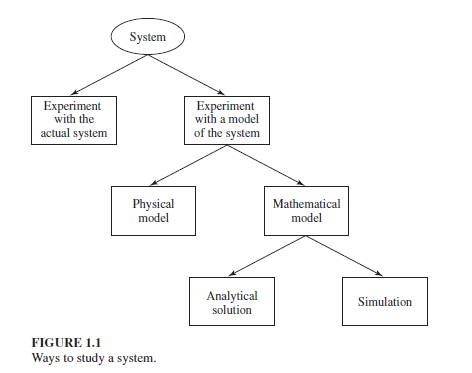
\includegraphics[width=8cm]{bilder/system_study}
	\caption{Arten von Systemstudien}
  \label{fig:sysstudy}
\end{figure}

\subsection{M/M/1-Modell}

\begin{figure}[h]
	\centering
	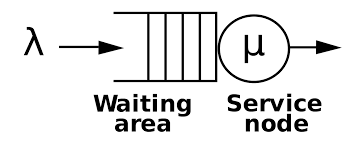
\includegraphics[width=8cm]{bilder/mm1}
	\caption{M/M/1 Warteschlangenmodell}
  \label{fig:mm1}
\end{figure}

% Verteilung der Zeitabstände zwischen Kunden
\begin{equation}
f_T(x) = \lambda e^{- \lambda t}, \quad t \geq 0
\end{equation}

% Verteilung der Zeitabstände zwischen Services
\begin{equation}
f_S(x) = \mu e^{- \mu t}, \quad t \geq 0
\end{equation}

\begin{figure}[h]
	\centering
	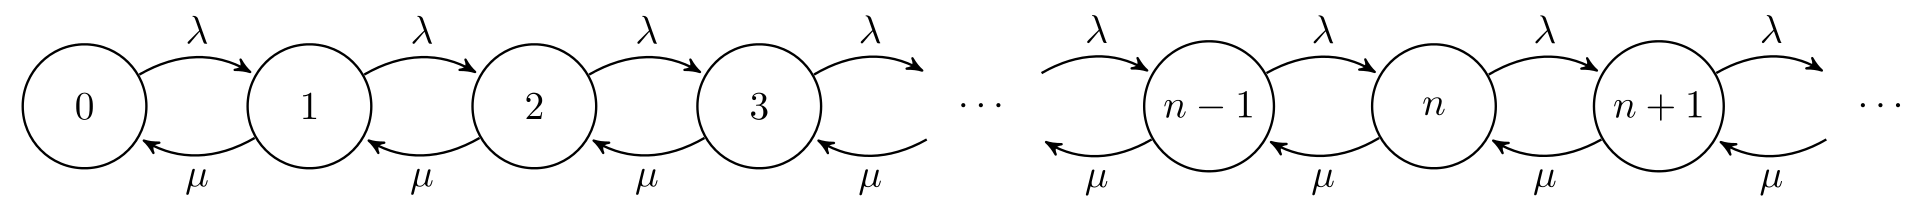
\includegraphics[width=8cm]{bilder/mm1_state}
	\caption{M/M/1 Zustandsübergangsdiagramm}
  \label{fig:mm1_state}
\end{figure}

% Verteilung für die Anzahl von Kunden im System
\begin{equation}
P_n = (1 - \rho) \rho^n
\end{equation}

% Erwartete Anzahl von Kunden im System
\begin{equation}
L = \frac{
	\rho
}{
	1 - \rho
} = \frac{
	\lambda
}{
	\mu - \lambda
}
\end{equation}

% Erwartete Wartezeit in der Queue
\begin{equation}
W_q = \frac{
	\rho
}{
	\mu - \lambda
} = \frac{
	\lambda
}{
	\mu ( \mu - \lambda )
}
\end{equation}

\section{Parameter-Schätzer}

% Regressionsfunktion
\begin{equation}
y_i = \eta(x_i, \theta)+ \epsilon_i, \quad i=1,2,...,n
\end{equation}

% Verteilung der Residuen
\begin{equation}
\epsilon \sim N(0, \sigma^2)
\end{equation}

% Erwartungswert der Daten soll die Regression sein
\begin{equation}
E(y | x) = \eta(x, \theta)
\end{equation}

% Schätzer
\begin{equation}
\hat{y} = \eta(x, \hat{\theta})
\end{equation}

% Kleinsten Quadrate
\begin{equation}
\underset{\theta \in \mathcal{R}}{\arg\min} \sum_{i=1}^n \left[ \eta(x_i,\theta) - y_i \right]^2
\end{equation}

% M estimator
\begin{equation}
\sum_{i=1}^n \psi(y_i, \theta) = 0
\end{equation}

\subsection{Maximum-Likelihood-Schätzer}

% Likelihood
\begin{equation}
\mathit{Lik}(\theta, y) = \prod_{i=1}^n f(y_i, \theta)
\end{equation}

% log Likelihood
\begin{equation}
L(\theta, y) = \log \prod_{i=1}^n f(y_i, \theta) = \sum_{i=1}^n \log f(y_i, \theta)
\end{equation}

\begin{equation}
\frac{\partial}{\partial \theta} L(\theta, y) = \sum_{i=1}^n \frac{\partial}{\partial \theta} \log f(y_i, \theta) = 0
\end{equation}

\begin{equation}
\psi = \frac{ -f }{ f }
\end{equation}

\begin{equation}
\mathrm{Var}(\theta) = \left[ I(\theta) \right]^{-1}
\end{equation}

\begin{equation}
I(\theta) = E \left(- \frac{\partial^2}{\partial \theta^2} L(\theta, y) \right) 
\end{equation}

\begin{equation}
\mathrm{Var}(\hat{\theta}) \approx \left[ \left. - \frac{\partial^2}{\partial \theta^2} L(\theta, y) \right|_{\theta = \hat{\theta}} \right]^{-1}
\end{equation}

\section{GoF-Tests}

\subsection{Kolmogorov-Smirnov Test}

\begin{equation}
D = \underset{y_i}{\sup} \{ F_n(y_i) - F(y_i, \theta) \}
\end{equation}

\subsection{Anderson-Darling Test}

\begin{equation}
A^2 = -n - \sum_{i=1}^n \frac{2 i - 1}{n} \left[ \log F(y_i, \hat{\theta}) + \log( 1 - F(y_{n+1-i}, \hat{\theta})) \right]
\end{equation}

\subsection{Chi-Quadrat Test}

\section{Konfidenzintervalle}

% Erwartete Wartezeit in der Queue für allgemeinere M/G/1 Systeme
\begin{equation}
W_q = \frac{
	\lambda \left[ \mathrm{Var}(S) + (E(S))^2 \right]
}{
	2 (1 - \lambda E(S)) 
}
\end{equation}

\section{Konfidenzbänder}

\section{Coverage Error}

\section{Resampling Verfahren}

\subsection{Bootstrap}
























% kapitel3.tex
\chapter{Vorstellung der Algorithmen}
\label{chapter:kap3}
Banks, J. 1998. Handbook of simulation: 
- 7.2.3: Quantile Estimation

Was sind Voraussetzungen, die durch Bootstrap abgelöst werden?



Es werden im wesentlich zwei Ansätze vorgestellt, die Resampling einsetzen, um Konfidenzbänder zu bestimmen.

Der erste Ansatz Setzt Bootstrap ein, um

\section{Standard Bootstrap}

\section{Bootstrapping der Residuen}

\section{Parametrsches Bootstrap}

\section{Wild Bootstrap}

\section{Bayes'sches Bootstrap}

\section{Resampling von $\partial R(\alpha)$}
Banks, J. 1998. Handbook of simulation: 
- 5: Random Variate Generation (S. 143 ff)
% kapitel4.tex
\chapter{Implementierung}
\label{chapter:kap4}

\section{OMNeT++}

\subsection{Überblick}

\subsection{Simulationen}

\section{Parameterstudien in OMNeT++}

\subsection{Datenerfassung}

\subsection{Auswertung}

\subsection{Darstellung}

\section{}
% kapitel5.tex
\chapter{Auswertung}
\label{chapter:kap5}

\section{Analytisches Verfahren}

\section{parametrisches Bootstrapping}

\section{nicht-parametrisches Bootstrapping}

\section{Vergleich}

% schlussteil.tex
\chapter{Schlussteil}

\section{Fazit}

\section{Ausblick}

% Anhang
\appendix
% anhang.tex
\chapter{Weitere Informationen}

% Abbildungsverzeichnis
\listoffigures
\addcontentsline{toc}{chapter}{Abbildungsverzeichnis}
\cleardoublepage
% Algorithmenverzeichnis
\listofalgorithms
\addcontentsline{toc}{chapter}{Algorithmenverzeichnis}
\cleardoublepage
% Literaturverzeichnis
\bibliographystyle{gerplain}
\bibliography{literatur/diplom}
\addcontentsline{toc}{chapter}{\bibname}
% Erklaerung
\thispagestyle{myheadings}
\markboth{}{ERKLÄRUNG}
\addcontentsline{toc}{chapter}{Erklärung}
% erklaerung.tex
\cleardoublepage
\normalsize
Hiermit versichere ich, dass ich die vorliegende Arbeit selbstständig verfasst habe und keine anderen als die angegebenen Quellen und Hilfsmittel verwendet sowie Zitate kenntlich gemacht habe.\\\\
Dortmund, den \today \\\\\\\\
Muster Mustermann
% EOF
\cleardoublepage
\end{document}

